% =====================================================================
%  Redes Neuronales 2026 (FaMAF-UNC) - Trabajo Práctico 1
%  Simulación numérica del modelo de neuronas de Izhikevich
%  Texto: versión final del grupo (.docx del 14/10/2026).
%  Figuras en figuras/. Compilar con pdfLaTeX (en Overleaf: Recompile).
% =====================================================================
\documentclass[10pt,a4paper,twocolumn]{article}

\usepackage[utf8]{inputenc}
\usepackage[T1]{fontenc}
\usepackage[spanish,es-tabla,es-noshorthands,es-nodecimaldot]{babel}
\usepackage{lmodern}
\usepackage[a4paper,margin=1.7cm,columnsep=0.65cm]{geometry}
\usepackage{microtype}
\usepackage{amsmath,amssymb}
\usepackage{icomma}
\usepackage{graphicx}
\graphicspath{{figuras/}}
\usepackage{booktabs}
\usepackage[font=small,labelfont=bf,labelsep=period,skip=4pt]{caption}
\usepackage{enumitem}
\usepackage{xcolor}
\usepackage[colorlinks=true,linkcolor=blue!50!black,citecolor=blue!50!black,urlcolor=blue!50!black]{hyperref}

\setlength{\textfloatsep}{8pt plus 2pt minus 2pt}
\setlength{\floatsep}{6pt plus 2pt minus 2pt}
\setlength{\dbltextfloatsep}{8pt plus 2pt minus 2pt}

\title{\vspace{-1.2cm}\textbf{Simulación numérica del modelo de neuronas de Izhikevich}}
\author{%
  Mariel Anachuri, Camila Giolitto, Martín Robins\\[2pt]
  \small Facultad de Matemática, Astronomía, Física y Computación, Universidad Nacional de Córdoba\\
  \small Redes Neuronales 2026
}
\date{\vspace{-0.6cm}}

\raggedbottom
\begin{document}

\twocolumn[{
  \begin{@twocolumnfalse}
    \maketitle
    \vspace{-0.4cm}
    \begin{abstract}
    \noindent
    En este trabajo se implementa y analiza el modelo de neuronas de disparo de
    Izhikevich, integrado con el método de Runge--Kutta de cuarto orden (RK4)
    con un paso $h = 0,1$~ms y una condición de reseteo aplicada cuando
    $v \geq 30$~mV. En primer lugar, se estudió la respuesta de una neurona con
    parámetros típicos ante un escalón de corriente. Luego, se reprodujeron ocho
    patrones de actividad neuronal: Regular Spiking (RS), Intrinsically Bursting (IB),
    Chattering (CH), Fast Spiking (FS), Low-Threshold Spiking (LTS), Thalamocortical
    (TC1 y TC2) y Resonator (RZ). Las simulaciones reproducen cualitativamente los
    patrones del artículo original y muestran que su diversidad está determinada por
    los parámetros del modelo y por la corriente de entrada. Por último, se analizó el
    efecto del paso de integración: los tiempos de disparo dependen de $h$ y su error
    se acumula con cada disparo debido al reseteo, sin alterar los patrones
    cualitativos.

    \smallskip\noindent
    \textbf{Palabras clave:} modelo de Izhikevich, simulación numérica, ecuaciones
    diferenciales, dinámica neuronal.
    \end{abstract}
    \vspace{0.4em}
  \end{@twocolumnfalse}
}]

% =====================================================================
\section{Introducción}

La modelización matemática y computacional constituye una herramienta fundamental
para estudiar el funcionamiento del sistema nervioso, ya que permite describir la
actividad neuronal y explorar los mecanismos que la sustentan. Como señalan Dayan y Abbott~\cite{dayan2001}, un modelo más detallado no es necesariamente superior: debe actuar
como puente entre distintos niveles de comprensión, incorporando suficiente
información para representar los mecanismos biológicos de interés y manteniendo la
simplicidad necesaria para facilitar su análisis.

Este equilibrio entre detalle y simplicidad se refleja en los modelos de neuronas de
disparo, que describen la evolución del potencial de membrana y la generación de
potenciales de acción en respuesta a corrientes de entrada. Los modelos
Integrate-and-Fire, derivados de la propuesta de Lapicque~\cite{lapicque1907}, representan la
integración de las corrientes de entrada y el disparo mediante un umbral, seguido de
un reseteo del potencial de membrana, sin describir en detalle el potencial de
acción. Esto facilita el análisis matemático y reduce el costo computacional de las
simulaciones \cite{dayan2001}. Por su parte, el modelo de Hodgkin--Huxley
incorpora las conductancias de sodio y potasio dependientes del voltaje, lo que
permite describir la generación y la evolución temporal del potencial de acción,
aunque requiere resolver un sistema de ecuaciones más complejo \cite{hodgkin1952}.

En este contexto, el modelo de Izhikevich combina la riqueza de las dinámicas
neuronales que caracteriza al modelo Hodgkin--Huxley con la eficiencia computacional
de los modelos Integrate-and-Fire. Su formulación se basa en la teoría de
bifurcaciones y la reducción a formas normales~\cite{izhikevich2003,izhikevich2007}, lo que permite conservar
características relevantes de la dinámica neuronal mediante una descripción
simplificada. A partir de dos ecuaciones diferenciales y una regla de reseteo,
reproduce distintos patrones de disparo y ráfagas mediante el ajuste de cuatro
parámetros, lo que facilita la simulación de redes neuronales de gran tamaño~\cite{izhikevich2003}.

El objetivo de este trabajo es estudiar la capacidad del modelo de Izhikevich para
reproducir distintos patrones de actividad neuronal mediante una descripción
matemática simplificada. Para ello, se realizaron simulaciones numéricas utilizando
el método de Runge--Kutta de cuarto orden y se analizó cómo los parámetros del modelo
y las corrientes de entrada influyen en el comportamiento neuronal, comparando los
patrones obtenidos con los presentados en el artículo original.

\begin{table*}[!t]
  \centering
  \caption{Parámetros, potencial inicial y corriente de entrada del caso base y de los
  ocho patrones simulados. En todos los casos, $u(0) = b\,v(0)$.}
  \label{tab:casos}
  \small\setlength{\tabcolsep}{4.5pt}
  \begin{tabular}{lcccccl}
    \toprule
    Caso & $a$ & $b$ & $c$ (mV) & $d$ & $v(0)$ (mV) & Corriente ($t$ en ms) \\
    \midrule
    Caso base & 0,02 & 0,20 & $-65$ & 2    & $-70$   & $I_0$: 0 ($t<10$); 10 ($t \geq 10$) \\
    RS        & 0,02 & 0,20 & $-65$ & 8    & $-65$   & $I_1$: 0 ($t<20$); 10 ($t \geq 20$) \\
    IB        & 0,02 & 0,20 & $-55$ & 4    & $-65$   & $I_1$: 0 ($t<20$); 10 ($t \geq 20$) \\
    CH        & 0,02 & 0,20 & $-50$ & 2    & $-65$   & $I_1$: 0 ($t<20$); 10 ($t \geq 20$) \\
    FS        & 0,10 & 0,20 & $-65$ & 2    & $-65$   & $I_1$: 0 ($t<20$); 10 ($t \geq 20$) \\
    TC1       & 0,02 & 0,25 & $-65$ & 0,05 & $-63$   & $I_2$: 0 ($t<20$); 1 ($t \geq 20$) \\
    TC2       & 0,02 & 0,25 & $-65$ & 0,05 & $-65$   & $I_3$: 0 ($t<20$); $-25$ ($20 \leq t < 80$); 0 ($t \geq 80$) \\
    RZ        & 0,10 & 0,26 & $-65$ & 2    & $-62,5$ & $I_4$: 0 ($t<40$); 0,2 ($40 \leq t < 180$); 2,2 ($180 \leq t < 181$); 0,2 ($t \geq 181$) \\
    LTS       & 0,02 & 0,25 & $-65$ & 2    & $-65$   & $I_1$: 0 ($t<20$); 10 ($t \geq 20$) \\
    \bottomrule
  \end{tabular}
\end{table*}

% =====================================================================
\section{Teoría y metodología numérica}

\subsection*{El modelo de Izhikevich}

Está descrito por el siguiente sistema de dos ecuaciones diferenciales ordinarias
(EDO):
\begin{align}
  \frac{dv}{dt} &= 0,04\,v^{2} + 5v + 140 - u + I, \label{eq:v}\\
  \frac{du}{dt} &= a\,(bv - u), \label{eq:u}
\end{align}
junto a un mecanismo de reseteo posterior al pico (\emph{after-spike reset}):
\begin{equation}
  \text{si } v \geq 30~\text{mV}, \quad
  \begin{cases}
    v \leftarrow c,\\
    u \leftarrow u + d.
  \end{cases}
  \label{eq:reset}
\end{equation}

\subsection*{Interpretación de las variables y los parámetros}

La dinámica del modelo se describe mediante dos variables de estado, una corriente de
entrada y cuatro parámetros que regulan el comportamiento de la neurona~\cite{izhikevich2003}.
\begin{itemize}[leftmargin=*,itemsep=1pt,topsep=2pt]
  \item $v$ (potencial de membrana): representa el potencial de membrana eléctrico de
  la neurona y se expresa en milivoltios (mV).
  \item $u$ (variable de recuperación): resume la activación de corrientes de potasio
  (K$^{+}$) y la inactivación de corrientes de sodio (Na$^{+}$). Proporciona una
  retroalimentación negativa sobre el potencial de membrana.
  \item $I$ (corriente de entrada): representa la corriente aplicada a la neurona, que
  puede ser inyectada directamente o corresponder a corrientes sinápticas.
  \item $a$ (escala temporal de $u$): determina la velocidad con la que evoluciona la
  variable de recuperación $u$. Los valores menores producen una recuperación más
  lenta. Un valor típico es $a = 0,02$.
  \item $b$ (sensibilidad de $u$ a $v$): describe cómo responde la variable $u$ a las
  fluctuaciones subumbrales de $v$. Los valores mayores acoplan más fuertemente ambas
  variables y pueden favorecer oscilaciones subumbrales y disparos de bajo umbral. Un
  valor típico es $b = 0,2$.
  \item $c$ (reseteo del potencial): establece el valor al que se restablece $v$
  después de alcanzar el pico del disparo ($+30$~mV). Se relaciona con la acción de
  las conductancias de potasio de activación rápida. Un valor típico es
  $c = -65$~mV.
  \item $d$ (salto de recuperación): determina el incremento instantáneo que se suma a
  la variable $u$ después de alcanzar el pico del disparo. Se relaciona con
  conductancias de sodio y potasio más lentas. Un valor típico es $d = 2$.
\end{itemize}

\subsection*{Condición de corte y umbral}

El valor de $+30$~mV no constituye un umbral de disparo fisiológico fijo, sino que se
utiliza como referencia para detectar el pico del potencial de acción y aplicar la
condición de reseteo.

A diferencia de los modelos Integrate-and-Fire (IF) tradicionales, que suelen emplear
un umbral fijo, el modelo de Izhikevich presenta un umbral efectivo de disparo
dinámico, que depende del estado previo de $v$ y $u$ y puede variar aproximadamente
entre $-55$~mV y $-40$~mV~\cite{izhikevich2003}.

\subsection*{Diversidad de patrones de disparo}

Mediante distintas combinaciones de los parámetros, el modelo nos permite reproducir
patrones de disparo característicos de diferentes tipos de neuronas corticales y
talámicas~\cite{izhikevich2003}. Entre ellas se encuentran las neuronas excitatorias
Regular Spiking (RS), Intrinsically Bursting (IB) y Chattering (CH); las interneuronas
inhibitorias Fast Spiking (FS) y Low-Threshold Spiking (LTS); los regímenes de
disparo tálamo-cortical tónico (TC1) y de ráfaga de rebote (TC2), y el patrón
Resonator (RZ) (Figura~\ref{fig:planos}).

\begin{figure}[t]
  \centering
  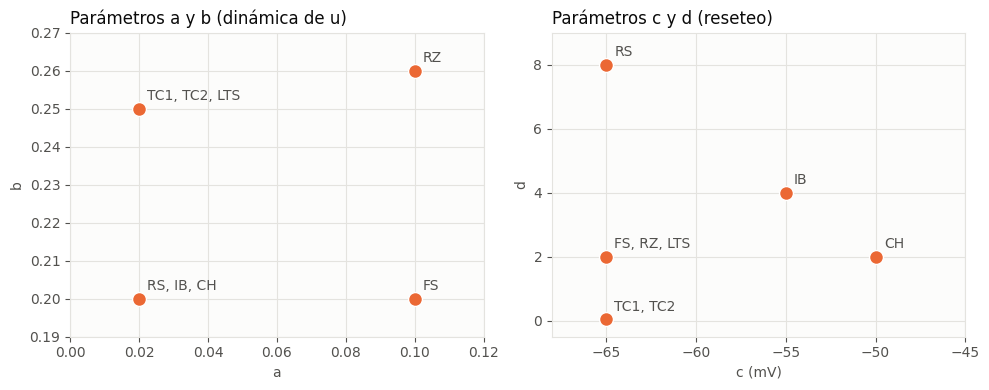
\includegraphics[width=\columnwidth]{fig1_planos.png}
  \caption{Ubicación de las ocho configuraciones utilizadas en el espacio de
  parámetros del modelo de Izhikevich.}
  \label{fig:planos}
\end{figure}

\begin{figure}[!b]
  \centering
  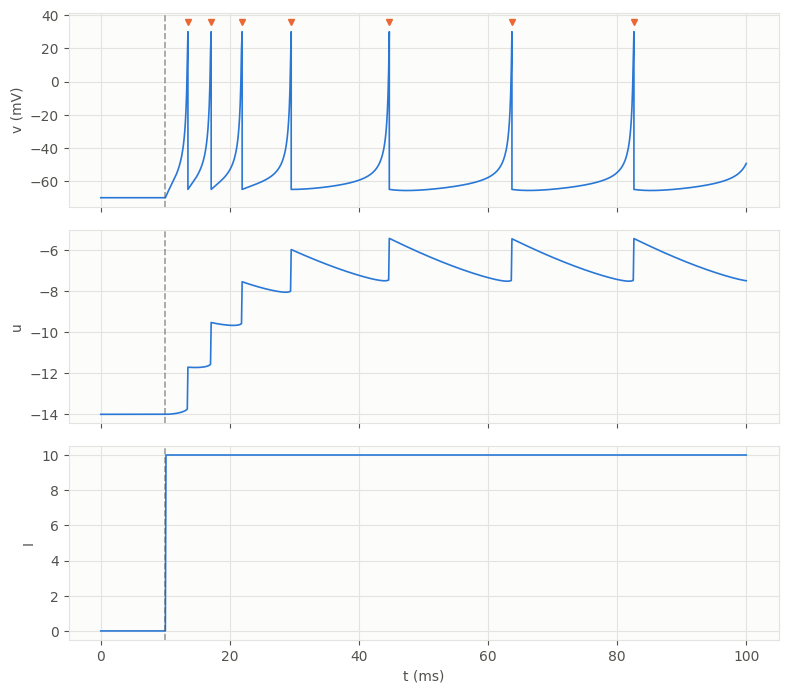
\includegraphics[width=\columnwidth]{fig2_caso_base.png}
  \caption{Evolución temporal del potencial de membrana $v(t)$, la variable de
  recuperación $u(t)$ y la corriente de entrada $I(t)$ (de arriba abajo). Para el
  caso base se aplicó un escalón de amplitud $I = 10$ desde $t = 10$~ms (línea
  punteada), con $a = 0,02$; $b = 0,2$; $c = -65$~mV; $d = 2$; $v(0) = -70$~mV y
  $u(0) = -14$. Los triángulos marcan los instantes de disparo. Integración con RK4
  y $h = 0,1$~ms.}
  \label{fig:base}
\end{figure}

\begin{figure*}[!t]
  \centering
  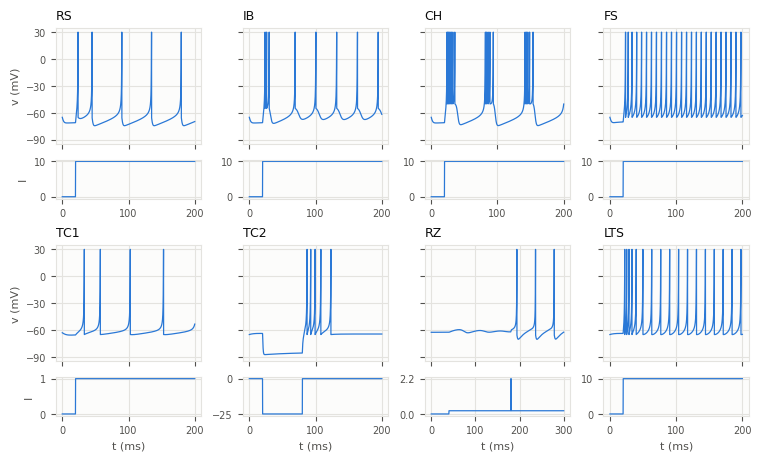
\includegraphics[width=0.82\textwidth]{fig3_ocho_tipos.png}
  \caption{Potencial de membrana $v(t)$ y corriente de entrada $I(t)$ (debajo de cada
  panel) para los ocho patrones: RS, IB, CH, FS, TC1, TC2, RZ y LTS (parámetros y
  protocolos en la Tabla~\ref{tab:casos}). Cada simulación dura 200~ms, salvo RZ
  (300~ms). Integración con RK4 y $h = 0,1$~ms.}
  \label{fig:ocho}
\end{figure*}

\subsection*{Integración numérica}

Las ecuaciones \eqref{eq:v} y \eqref{eq:u} se integraron numéricamente con el método
de Runge--Kutta de cuarto orden (RK4), implementado en Python, con un paso de
integración de $h = 0,1$~ms. Dado el estado $x = (v, u)$ en el instante $t$, el
estado en $t + h$ se calcula como
\begin{equation}
  x(t + h) = x(t) + \frac{h}{6}\,(k_{1} + 2k_{2} + 2k_{3} + k_{4}),
\end{equation}
con $k_1 = f(x, t)$, $k_2 = f(x + h k_1/2,\, t + h/2)$,
$k_3 = f(x + h k_2/2,\, t + h/2)$ y $k_4 = f(x + h k_3,\, t + h)$, donde $f$ denota el
lado derecho de las ecuaciones \eqref{eq:v} y \eqref{eq:u}.

Después de cada paso de integración se verifica si $v \geq 30$~mV; en ese caso se
registra el instante del disparo y se aplica de inmediato el reseteo
\eqref{eq:reset}. Como condiciones iniciales se usó $u(0) = b\,v(0)$, con los valores
de $v(0)$ indicados en la Tabla~\ref{tab:casos}. El intervalo de integración fue
$[0, 100]$~ms para el caso base y 200~ms para los patrones (300~ms para RZ, cuyo
pulso ocurre a los 180~ms). Para evaluar el error numérico, el caso base se repitió
con $h = 0,2$; $0,05$ y $0,01$~ms, y se tomó $h = 0,01$~ms como referencia.

% =====================================================================
\section{Resultados}

\subsection*{Respuesta neuronal a un escalón de corriente}

Se analizó inicialmente la respuesta del caso base a un escalón de corriente aplicado
en $t = 10$~ms. La Figura~\ref{fig:base} muestra la evolución del potencial de
membrana y de la variable de recuperación, junto con la corriente de entrada. Hasta
la aplicación del estímulo la neurona permanece en reposo ($v = -70$~mV). Luego se
observa un tren de disparos, el primero en 13,5~ms, cuyos intervalos entre disparos
consecutivos aumentan progresivamente de 3,6~ms a unos 19~ms hasta alcanzar un
régimen aproximadamente periódico. Cada disparo está acompañado por un incremento de
$u$ de valor $d = 2$, seguido por una evolución continua entre eventos.

\subsection*{Dinámicas neuronales para distintas configuraciones}

La Figura~\ref{fig:ocho} presenta la respuesta de las ocho configuraciones de
parámetros correspondientes a los distintos tipos neuronales. RS, IB, CH, FS y LTS
reciben el mismo escalón de corriente ($I = 10$) a partir de los 20~ms, por lo que sus
diferentes respuestas se deben exclusivamente a la modificación de los parámetros del
modelo. RS, FS y LTS producen disparos individuales, con frecuencias y evoluciones
distintas. RS dispara a baja frecuencia: luego de un primer intervalo más corto, los
siguientes se espacian y mantienen un período constante. LTS, en cambio, comienza
disparando a alta frecuencia y sus intervalos crecen progresivamente hasta
estabilizarse. FS es la de mayor frecuencia y mantiene intervalos prácticamente
constantes durante todo el estímulo. IB y CH, por su parte, responden con ráfagas. En
IB hay una ráfaga inicial seguida de disparos aislados de forma regular, mientras que
en CH las ráfagas se repiten a intervalos aproximadamente regulares durante todo el
estímulo.

La neurona tálamo-cortical responde de dos formas distintas según el estímulo que
recibe. En TC1, una corriente débil y constante ($I = 1$) hace que la neurona dispare
de a uno, con disparos bien separados entre sí. En TC2, la corriente es negativa:
mientras se aplica, el potencial baja por debajo del reposo, y cuando se retira, la
neurona responde con una ráfaga de disparos antes de volver al reposo.

Por último, en RZ una corriente pequeña hace que el potencial oscile levemente, pero
sin llegar a disparar. Recién cuando se aplica un pulso breve a los 180~ms, la
neurona empieza a disparar de forma repetida.

\begin{figure}[t]
  \centering
  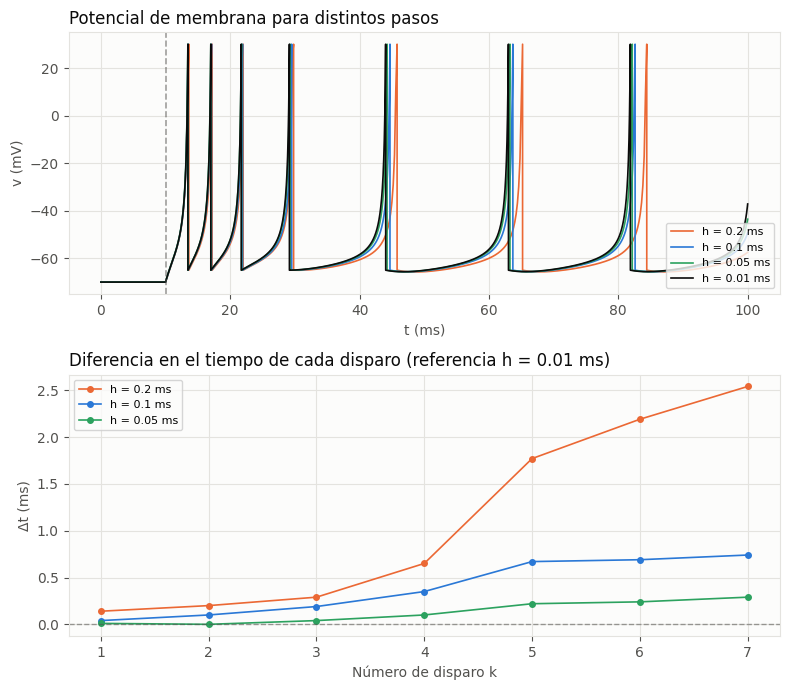
\includegraphics[width=\columnwidth]{fig4_error.png}
  \caption{Efecto del paso de integración sobre el caso base. Arriba: potencial de
  membrana para $h = 0,2$; $0,1$; $0,05$ y $0,01$~ms. Abajo: diferencia en el tiempo
  del $k$-ésimo disparo respecto de la simulación de referencia con $h = 0,01$~ms. La
  línea punteada marca el inicio del estímulo.}
  \label{fig:error}
\end{figure}

La Figura~\ref{fig:error} muestra el efecto del paso de integración sobre el caso
base. Con los cuatro pasos se obtienen siete disparos, pero sus tiempos se desplazan:
con el paso más grande ($h = 0,2$~ms) los disparos se retrasan respecto de la
referencia. Esa diferencia crece con el número de disparos, es decir, el error se
acumula a lo largo de la simulación, con un aumento marcado entre el cuarto y el
quinto disparo. En el último disparo el desfase es de 2,5~ms con $h = 0,2$~ms, de
0,7~ms con $h = 0,1$~ms y de 0,3~ms con $h = 0,05$~ms. Cuanto menor es el paso, menor
es el desfase.

% =====================================================================
\section{Discusión}

Las simulaciones reproducen cualitativamente los ocho patrones de la Figura~2 de
Izhikevich~\cite{izhikevich2003}. Sus diferencias se explican por cómo los parámetros regulan el
freno que $u$ ejerce sobre $v$. Un $d$ grande refuerza el freno con cada disparo y
produce adaptación (RS); un $a$ grande lo libera rápido y evita la adaptación (FS); y
un $c$ alto deja a $v$ cerca del disparo tras el reseteo, lo que genera ráfagas que se
repiten o no según el valor de $d$ (CH e IB). En TC2, la corriente negativa reduce
también $u$, por lo que al retirarla la neurona queda con poco freno y dispara. RZ
muestra la biestabilidad entre reposo y disparo repetitivo descripta en el artículo.
Como los protocolos de TC1, TC2 y RZ son propios del práctico, la comparación en esos
casos es cualitativa. Estos casos muestran además que la diversidad de
comportamientos no depende solo de los parámetros, sino también de la corriente de
entrada, ya que una misma neurona puede responder de manera distinta según el
estímulo que recibe.

En cuanto a la integración numérica (Figura~\ref{fig:error}), la principal fuente de
error es el reseteo: el disparo se detecta al final del paso en que $v$ supera los
30~mV, con un error de hasta un paso $h$, y como cada disparo parte del reseteo
anterior, estos desfases se acumulan. Por eso, aunque RK4 es de cuarto orden, el
reseteo limita la precisión de los tiempos de disparo. Con $h = 0,1$~ms, el paso que
usa el artículo, el desfase no altera los patrones, aunque los tiempos de disparo
dependen del paso elegido.

En síntesis, con solo dos ecuaciones diferenciales y cuatro parámetros, el modelo de
Izhikevich reproduce una amplia variedad de comportamientos neuronales sin describir
en detalle los mecanismos biofísicos que los originan. Esto lo ubica en el punto
intermedio entre detalle y simplicidad que plantean Dayan y Abbott~\cite{dayan2001}, y hace
posible su uso en la simulación de redes con un gran número de neuronas~\cite{izhikevich2003}.

% =====================================================================
\begin{thebibliography}{9}\small
\setlength{\itemsep}{1pt}
\bibitem{dayan2001}
  P.~Dayan and L.~F. Abbott, \emph{Theoretical Neuroscience: Computational and
  Mathematical Modeling of Neural Systems} (MIT Press, Cambridge, MA, 2001).
\bibitem{lapicque1907}
  L.~Lapicque, Recherches quantitatives sur l'excitation électrique des nerfs
  traitée comme une polarisation, J. Physiol. Pathol. Gen. \textbf{9}, 620--635
  (1907).
\bibitem{hodgkin1952}
  A.~L. Hodgkin and A.~F. Huxley, A quantitative description of membrane current and
  its application to conduction and excitation in nerve, J. Physiol. \textbf{117},
  500--544 (1952).
\bibitem{izhikevich2003}
  E.~M. Izhikevich, Simple model of spiking neurons, IEEE Trans. Neural Netw.
  \textbf{14}, 1569--1572 (2003).
\bibitem{izhikevich2007}
  E.~M. Izhikevich, \emph{Dynamical Systems in Neuroscience: The Geometry of
  Excitability and Bursting} (MIT Press, Cambridge, MA, 2007).
\end{thebibliography}

\end{document}
